\documentclass[10pt,a4paper]{article}
\usepackage[utf8]{inputenc}
\usepackage[spanish]{babel}
\usepackage{a4wide}
\usepackage[sinEntregas]{caratula}
\usepackage{ulem}
\usepackage{marginnote}
\usepackage{fancyhdr}
\usepackage{lastpage}
\usepackage{float}
\usepackage{tikz}

\pagestyle{fancy}
\thispagestyle{fancy}
\addtolength{\headheight}{1pt}
\lhead{TP2}
\rhead{Bases de Datos}
\cfoot{\thepage /\pageref{LastPage}}
\renewcommand{\thesubsubsection}{\thesubsection.\alph{subsubsection}}

\title{Bases de Datos - TP 2}
\author{Bases de Datos, DC, UBA.}

\begin{document}

\fecha{Bases de Datos}

\materia{Informe Ejecutivo}
%\submateria{Trabajo Pr\'actico Nº1}
\titulo{Web Semántica}

\integrante{Allocati, Federico}{682/11}{fede.allocati@gmail.com}
\integrante{Izcovich, Sabrina}{550/11}{sizcovich@gmail.com}
\integrante{Pernigotti, Santiago}{870/11}{spernigotti@hotmail.com}
\integrante{Romano, Germán}{786/11}{romano.german@live.com.ar}

\maketitle

\tableofcontents

\newpage

\section{Introducción}

El siguiente informe consiste en un análisis enfocado en la \textit{Web Semántica}. Para la realización del mismo, basamos nuestra investigación en la tesis\footnote{http://dc.uba.ar/inv/tesis/licenciatura/2013/bursztyn.pdf} presentada por \textit{Damián A. Bursztyn} en el año 2013 sobre \textbf{Optimización de consultas RDF reformuladas} y en el artículo \textbf{Introduction to the Special Issue on Semantic Web Data Management} escrito por \textit{Roberto De Virgilio} en 2011.

En lo que sigue, explicaremos los conceptos de Web Semántica y sus problemáticas, de su formato de representación \textit{RDF} y de los mecanismos que ayuda a convertir la Web en una infraestructura global en la que es posible compartir, y reutilizar datos y documentos entre diferentes tipos de usuarios.

\section{Web Semántica}
La Web Semántica consiste en una Web Extendida dotada de mayor significado gracias a los metadatos que acompañan a los datos que circulan. Su utilidad principal es encontrar soluciones a problemas habituales en la búsqueda de información gracias a la utilización de una infraestructura común mediante la que se procesa y transfiere información de una manera sencilla. Esta Web extendida y basada en el \textit{significado}, se apoya en lenguajes universales que resuelven los problemas ocasionados por una Web carente de semántica en la que, en ocasiones, el acceso a la información se convierte en una tarea difícil.

En lo que sigue, veamos un ejemplo de un buscador en la Web Semántica:

\begin{figure}[H] %[h] Aqui [b] para button [t] para top
\begin{center}
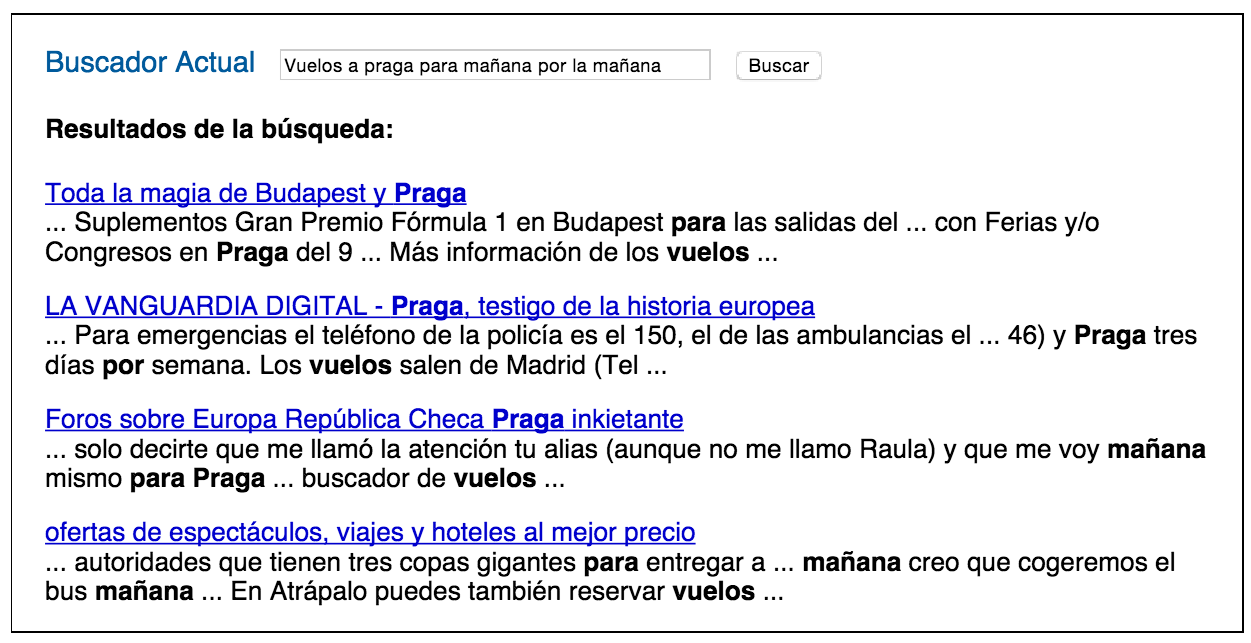
\includegraphics[width=400pt]{imgs/resultadoNormal}
\caption{Resultados obtenidos con un buscador normal.}
\end{center}
\end{figure}
\begin{figure}[H] %[h] Aqui [b] para button [t] para top
\begin{center}
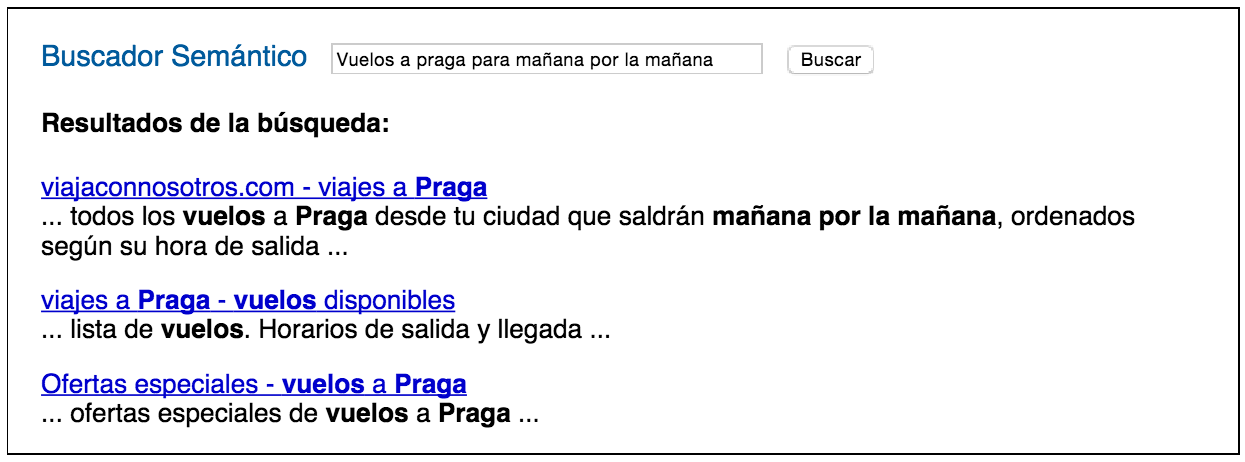
\includegraphics[width=400pt]{imgs/resultadoSemantico}
\caption{Resultados obtenidos con un buscador semántico.}
\end{center}
\end{figure}

\section{RDF}
El principal formato de los datos de la Web Semántica es \textit{RDF}. Un set de datos \textit{RDF} consiste en datos explícitos e implícitos presentes en la base de datos, dados por restricciones semánticas. Éstos son obtenidos por un proceso que considera todas las restricciones para inferir las posibles consecuencias de la base de datos existente.

Principalmente, proporcionan información descriptiva simple sobre los recursos que se encuentran en la Web y que se utiliza, por ejemplo, en catálogos de libros, directorios, colecciones personales de música, fotos, eventos, etc.

\section{Problemas de la Web Semántica}
En el último tiempo, el uso de Web Semántica creció enormemente e impulsó la necesidad de emplear técnicas eficientes y escalables para responder a las consultas sobre una gran cantidad de datos heterogéneos. Una posible solución a este problema consiste en traducir las consultas en \textit{RDF} en consultas \textit{SQL} para ejecutarlas en los sistemas de gestión de bases de datos relacionales (RDBMS). Sin embargo, las bases de datos para Web Semántica complican a las tecnologías clásicas de gestión de datos que no tienen en cuenta los datos implícitos durante la evaluación de consultas. Una solución a esto es reformular la consulta entrante para luego traducirla en una consulta SQL que, al ser evaluada por el RDBMS, devuelve las respuestas completas. El problema de esto es que no se logra un buen rendimiento debido a la longitud sintáctica de las consultas SQL que resultan de reformulación. Dado que los RDBMSs no son capaces de optimizar eficientemente las consultas, por lo que en algunos casos fallan o registran tiempos elevados de evaluación.

%%\section{RDF y RDBMS}
%%Las consultas RDF se pueden transformar en consultas de bases de datos relacionales sin mucha dificultad. A partir de la consulta transformada es posible utilizar cualquiera de las dos métodos de vinculación de RDF para resolverla, saturación o reformulación.
%%\\\\
%%\textbf{Saturación:} Transforma los datos implícitos en explícitos, ampliando asi la base de datos. 
%%\\\\
%%\textbf{Reformulación:} Se reformula la consulta basandose en las restricciones conocidas antes de evaluarla. La ventaja principal es que se aplica por consulta y no a toda la base de datos.

\section{Mecanismos de conversión de la Web}
Para obtener una adecuada definición de los datos, la Web Semántica utiliza esencialmente OWL, SPARQL, BGP y RDF. Estos mecanismos ayudan a convertir la Web en una infraestructura global en la que es posible compartir, y reutilizar datos y documentos entre diferentes tipos de usuarios.
\begin{itemize}
\item \textbf{SPARQL} es lenguaje de consulta sobre RDF, que permite hacer búsquedas sobre los recursos de la Web Semántica utilizando distintas fuentes datos.
\item \textbf{BGP} es el Patrón de grafo básico.
\begin{itemize}
\item Las consultas BGP son un subconjunto del lenguaje de consultas SPARQL W3C para RDF. 
\item El mismo se corresponde con la clase de familias de consultas conjuntivas de las bases de datos relacionales. 
\item Conforman las consultas SPARQL más utilizadas en el mundo real.
\item Están compuestas por un conjunto de variables distinguidas, la cabeza y el conjunto de patrones de tripla (los BGP).
\end{itemize}

\item \textbf{OWL} es un mecanismo para desarrollar temas o vocabularios específicos en los que asociar esos recursos. Lo que hace OWL es proporcionar un lenguaje para definir ontologías estructuradas que pueden ser utilizadas a través de diferentes sistemas. Las ontologías, que se encargan de definir los términos utilizados para describir y representar un área de conocimiento, son utilizadas por los usuarios, las bases de datos y las aplicaciones que necesitan compartir información específica, es decir, en un campo determinado como puede ser el de las finanzas, medicina, deporte, etc. Las ontologías incluyen definiciones de conceptos básicos en un campo determinado y la relación entre ellos.
\end{itemize}

\section{Reformulación}

Las bases de datos para Web Semántica presentan datos implícitos que las RDBMs no tienen en cuenta a la hora de resolver las consultas.

Para solucionarlo, se aplican técnicas de \textbf{Reformulación} a la consulta entrante para luego traducirla a una consulta SQL que, al ser evaluada por el RDBMs devuelve la respuesta completa.

\section{Referencias}

\begin{itemize}
\item The World Wide Web Consortium (W3C). http://www.w3c.es/Divulgacion/GuiasBreves/WebSemantica
\item http://jplu.developpez.com/tutoriels/web-semantique/introduction/
\item W3C Recommendation. http://www.w3.org/TR/rdf-sparql-query/
\end{itemize}

\end{document}